% ============================================================
%  CS3401 – Chapter 4: Decrease & Conquer + Divide & Conquer
%  (Merged from classic Chapters 4 and 5)
% ============================================================
\documentclass[aspectratio=169]{beamer}
% ============================================================
%  CS3401 – Algorithm Design and Analysis
%  Shared Beamer Theme (input this file in every chapter)
%  Prince Sattam Bin Abdulaziz University – CCES
% ============================================================

% ---------- PACKAGES ----------------------------------------
\usepackage[utf8]{inputenc}
\usepackage[T1]{fontenc}
\usepackage{lmodern}
\usepackage{amsmath,amssymb,amsthm}
\usepackage{tikz}
\usepackage{pgfplots}
\usepackage{booktabs}
\usepackage{xcolor}
\usepackage{graphicx}
\usepackage{listings}
\usepackage[normalem]{ulem}
\usepackage{algorithm}
\usepackage{algpseudocode}
\usepackage{multicol}
\usepackage{array}
\usepackage{colortbl}
\usepackage{tabularx}
\usepackage{makecell}

\usetikzlibrary{
  arrows.meta, shapes.geometric, shapes.symbols,
  positioning, calc, fit, backgrounds,
  decorations.pathreplacing, decorations.markings,
  matrix, chains, trees
}
\pgfplotsset{compat=1.18}

% ---------- COLOR PALETTE -----------------------------------
\definecolor{PrimaryDark}{RGB}{10,72,92}
\definecolor{PrimaryMid}{RGB}{18,114,145}
\definecolor{PrimaryLight}{RGB}{185,224,238}
\definecolor{AccentOrange}{RGB}{210,103,22}
\definecolor{AccentYellow}{RGB}{252,198,40}
\definecolor{SuccessGreen}{RGB}{32,122,66}
\definecolor{AlertRed}{RGB}{172,46,46}
\definecolor{CodeBg}{RGB}{244,246,250}
\definecolor{DarkText}{RGB}{28,32,40}
\definecolor{LightRule}{RGB}{210,225,232}
\tikzset{processstep/.style={draw=PrimaryMid, fill=PrimaryLight!35, rounded corners=2pt,
  align=center, minimum width=4.2cm, minimum height=0.55cm, font=\small}}

% ---------- BEAMER SETTINGS ---------------------------------
\setbeamertemplate{navigation symbols}{}
\setbeamertemplate{caption}[numbered]

% Fonts
\setbeamerfont{normal text}{size=\small}
\setbeamerfont{title}{series=\bfseries,size=\LARGE}
\setbeamerfont{subtitle}{series=\normalfont,size=\large}
\setbeamerfont{frametitle}{series=\bfseries,size=\large}
\setbeamerfont{framesubtitle}{series=\normalfont,size=\small}
\setbeamerfont{block title}{series=\bfseries,size=\normalsize}
\setbeamerfont{footline}{size=\tiny}
\addtobeamertemplate{frame begin}{\small\enlargethispage{1cm}}{}
\setlength{\tabcolsep}{2pt}

% Colors
\setbeamercolor{normal text}{fg=DarkText,bg=white}
\setbeamercolor{frametitle}{bg=PrimaryDark,fg=white}
\setbeamercolor{title}{fg=white}
\setbeamercolor{subtitle}{fg=PrimaryLight}
\setbeamercolor{author}{fg=white}
\setbeamercolor{date}{fg=PrimaryLight}
\setbeamercolor{institute}{fg=PrimaryLight}
\setbeamercolor{block title}{bg=PrimaryMid,fg=white}
\setbeamercolor{block body}{bg=PrimaryLight!35,fg=DarkText}
\setbeamercolor{block title alerted}{bg=AlertRed,fg=white}
\setbeamercolor{block body alerted}{bg=AlertRed!12,fg=DarkText}
\setbeamercolor{block title example}{bg=SuccessGreen,fg=white}
\setbeamercolor{block body example}{bg=SuccessGreen!12,fg=DarkText}
\setbeamercolor{itemize item}{fg=PrimaryMid}
\setbeamercolor{itemize subitem}{fg=AccentOrange}
\setbeamercolor{enumerate item}{fg=PrimaryMid}
\setbeamercolor{enumerate subitem}{fg=AccentOrange}
\setbeamercolor{alerted text}{fg=AlertRed}
\setbeamercolor{structure}{fg=PrimaryMid}
\setbeamercolor{section in toc}{fg=PrimaryDark}
\setbeamercolor{section in toc shaded}{fg=PrimaryDark}
% override Beamer's transparency-based shading so TOC entries stay fully visible
\setbeamertemplate{section in toc shaded}{\inserttocsection\par}
\setbeamercolor{subsection in toc}{fg=PrimaryMid}
\setbeamercolor{footer rule}{bg=LightRule}

% Item symbols
\setbeamertemplate{itemize item}{%
  \scriptsize\raise1.5pt\hbox{\color{PrimaryMid}$\blacktriangleright$}}
\setbeamertemplate{itemize subitem}{%
  \scriptsize\raise1pt\hbox{\color{AccentOrange}$\bullet$}}
\setbeamertemplate{itemize subsubitem}{%
  \scriptsize\raise1pt\hbox{\color{PrimaryDark}$\circ$}}
\setbeamertemplate{enumerate item}{%
  \color{PrimaryMid}\textbf{\insertenumlabel.}}

% Frame title
\makeatletter
\setbeamertemplate{frametitle}{%
  \nointerlineskip
  \begin{beamercolorbox}[wd=\paperwidth,ht=2.4em,dp=0.9em,%
                         leftskip=1.2em,rightskip=1.2em]{frametitle}
    \usebeamerfont{frametitle}\insertframetitle\strut
    \ifx\insertframesubtitle\@empty\else
      \hspace{0.6em}\textcolor{PrimaryLight!80}{\footnotesize|}\hspace{0.4em}%
      {\usebeamerfont{framesubtitle}\textcolor{PrimaryLight}\insertframesubtitle}%
    \fi
  \end{beamercolorbox}
  \nointerlineskip
  \begin{beamercolorbox}[wd=\paperwidth,ht=0.3pt,dp=0pt]{structure}
  \end{beamercolorbox}
}
\makeatother

% Footer
\setbeamertemplate{footline}{%
  \begin{beamercolorbox}[wd=\paperwidth,ht=0.4pt,dp=0pt]{footer rule}{}
  \end{beamercolorbox}
  \leavevmode
  \hbox{%
    \begin{beamercolorbox}[wd=0.60\paperwidth,ht=1.8em,dp=0.6em,leftskip=1em]{normal text}%
      \textcolor{PrimaryDark}{\tiny\textbf{CS3401} \textendash{} Algorithm Design \& Analysis%
        \quad\textbar\quad CCES, PSAU}%
    \end{beamercolorbox}%
    \begin{beamercolorbox}[wd=0.40\paperwidth,ht=1.8em,dp=0.6em,rightskip=1em,right]{normal text}%
      \textcolor{PrimaryDark}{\tiny\insertshorttitle%
        \quad\textbar\quad\insertframenumber\,/\,\inserttotalframenumber}%
    \end{beamercolorbox}%
  }%
}

% Title page
\setbeamertemplate{title page}{%
  
\begin{tikzpicture}[remember picture,overlay]
    \fill[PrimaryDark](current page.north west) rectangle (current page.south east);
    \fill[PrimaryMid,opacity=0.45]
      ([shift={(2.5cm,-2.5cm)}]current page.north east) circle(5.5cm);
    \fill[AccentOrange,opacity=0.10]
      ([shift={(-1.5cm,2.0cm)}]current page.south west) circle(4.2cm);
    \draw[white,opacity=0.08,line width=40pt]
      ([shift={(0cm,-0.5cm)}]current page.north west)
      to[out=-30,in=210]
      ([shift={(0cm,0.5cm)}]current page.south east);
  \end{tikzpicture}%
  \vspace{0.7cm}
  \begin{center}
    {\tiny\textcolor{PrimaryLight}{\textbf{CCES} \textendash{}
      College of Computer Engineering and Sciences}}\\[0.2em]
    {\tiny\textcolor{PrimaryLight}{Prince Sattam Bin Abdulaziz University}}\\[1.2em]
    {\footnotesize\textcolor{AccentYellow}{\textbf{CS3401 \textendash{} Algorithm Design and Analysis}}}\\[1.5em]
    \textcolor{PrimaryMid}{\rule{0.55\textwidth}{0.6pt}}\\[0.9em]
    {\Large\usebeamerfont{title}\textcolor{white}{\inserttitle}}\\[0.4em]
    {\small\usebeamerfont{subtitle}\textcolor{PrimaryLight}{\insertsubtitle}}\\[0.7em]
    \textcolor{PrimaryMid}{\rule{0.55\textwidth}{0.6pt}}\\[1.2em]
    {\footnotesize\textcolor{PrimaryLight}{\insertdate}}\\[0.6em]
    % Instructors row
    \begin{tikzpicture}[baseline=(current bounding box.center)]
      % Dr. Khalil – rounded photo
      \begin{scope}
        \clip (-3.2,0) circle (0.58cm);
        \node at (-3.2,0)
          {
\includegraphics[width=1.16cm,height=1.16cm,keepaspectratio=false]{khalil}};
      \end{scope}
      \draw[white,line width=0.9pt] (-3.2,0) circle (0.58cm);
      \node[text=white,font=\scriptsize\bfseries,anchor=west] at (-2.54,0)
        {Dr.\ Khalil Chebil};
      % Dr. Esraa – placeholder circle
      \draw[white,line width=0.9pt] (1.2,0) circle (0.58cm);
      \node[text=PrimaryLight,font=\normalsize\bfseries] at (1.2,0) {E};
      \node[text=white,font=\scriptsize\bfseries,anchor=west] at (1.86,0)
        {Dr.\ Esraa};
    \end{tikzpicture}
  \end{center}%
}

% Auto section-divider slide — background set via Beamer color system for reliability
\AtBeginSection[]{%
  {%
    \setbeamercolor{background canvas}{bg=PrimaryDark}%
    \begin{frame}[plain,noframenumbering]
      \begin{tikzpicture}[remember picture,overlay]
        \fill[PrimaryMid,opacity=0.35]
          ([shift={(0cm,-1.5cm)}]current page.north) circle(6.5cm);
        \node[text=white,opacity=0.06,font=\fontsize{120}{120}\bfseries]
          at ([shift={(-1cm,0cm)}]current page.center)
          {\insertsectionnumber};
      \end{tikzpicture}
      \vfill
      \begin{center}
        {\large\textcolor{AccentYellow}{\textbf{Section \insertsectionnumber}}}\\[0.6em]
        {\LARGE\textcolor{white}{\textbf{\insertsectionhead}}}
      \end{center}
      \vfill
    \end{frame}
  }%
}

% ---------- LISTINGS STYLE ----------------------------------
\lstset{
  basicstyle=\ttfamily\footnotesize,
  backgroundcolor=\color{CodeBg},
  keywordstyle=\color{PrimaryMid}\bfseries,
  commentstyle=\color{SuccessGreen}\itshape,
  stringstyle=\color{AccentOrange},
  numberstyle=\tiny\color{gray!70},
  frame=tb,
  framerule=0.5pt,
  rulecolor=\color{PrimaryLight},
  numbers=left,
  numbersep=6pt,
  showstringspaces=false,
  breaklines=true,
  tabsize=2,
  xleftmargin=1.8em,
  framexleftmargin=1.8em,
  captionpos=b,
  language=Java,
  morekeywords={var,let,const}
}

% ---------- PSEUDOCODE STYLE --------------------------------
\algrenewcommand\algorithmicprocedure{\textbf{Algorithm}}
\algrenewcommand\algorithmicfunction{\textbf{Function}}
\algrenewcommand\algorithmicif{\textbf{if}}
\algrenewcommand\algorithmicelse{\textbf{else}}
\algrenewcommand\algorithmicthen{\textbf{then}}
\algrenewcommand\algorithmicwhile{\textbf{while}}
\algrenewcommand\algorithmicfor{\textbf{for}}
\algrenewcommand\algorithmicforall{\textbf{for all}}
\algrenewcommand\algorithmicreturn{\textbf{return}}
\algrenewcommand\algorithmicend{\textbf{end}}
\algrenewcommand\algorithmicdo{}
\algrenewcommand\algorithmicrequire{\textbf{Input:}}
\algrenewcommand\algorithmicensure{\textbf{Output:}}

% ---------- CUSTOM COMMANDS ---------------------------------
\newcommand{\bigO}[1]{$\mathcal{O}(#1)$}
\newcommand{\bigTheta}[1]{$\Theta(#1)$}
\newcommand{\bigOmega}[1]{$\Omega(#1)$}
\newcommand{\highlight}[1]{\colorbox{AccentYellow!55}{\strut #1}}
\newcommand{\important}[1]{\textcolor{AlertRed}{\bfseries #1}}
\newcommand{\keyword}[1]{\textcolor{PrimaryMid}{\bfseries #1}}
\newcommand{\concept}[1]{\textcolor{AccentOrange}{\bfseries #1}}

% Colored table column types
\newcolumntype{H}{>{\columncolor{PrimaryDark}\color{white}\bfseries\centering\arraybackslash}m{2.5cm}}
\newcolumntype{Z}{>{\columncolor{PrimaryLight!40}\centering\arraybackslash}m{2cm}}

% Reference boxes
\newcommand{\refbox}[1]{%
  \begin{beamercolorbox}[rounded=true,shadow=false,leftskip=0.5em,rightskip=0.5em,%
                          ht=1.6em,dp=0.5em]{block title}
    \small\textit{Reference:} #1
  \end{beamercolorbox}%
}

% Inline complexity tag
\newcommand{\ctag}[1]{%
  \hfill\tikz[baseline]{\node[fill=AlertRed,text=white,rounded corners=2pt,
    font=\bfseries\scriptsize,inner sep=2pt,outer sep=0pt]{$\mathcal{O}(#1)$};}%
}


\title[Ch.\,4 -- Recursive Strategies]{Chapter 4}
\subtitle{Decrease \& Conquer and Divide \& Conquer}
\date{Academic Year 2026\,--\,2027}

\begin{document}

\begin{frame}[plain]\titlepage\end{frame}
\begin{frame}[shrink=20]{Chapter Overview}
  \begin{center}
    \begin{minipage}{0.85\textwidth}
      \tableofcontents[hideallsubsections,sectionstyle=show/shaded]
    \end{minipage}
  \end{center}
\end{frame}

% ============================================================
\section{Recursive Reduction — A Unified View}
% ============================================================

\begin{frame}[shrink=12]{Two Sides of the Same Coin}
  Both strategies rely on \keyword{recursive reduction}:
  \emph{solve a large instance by solving one or more smaller instances}.

  \vspace{0.5em}
  \begin{center}
  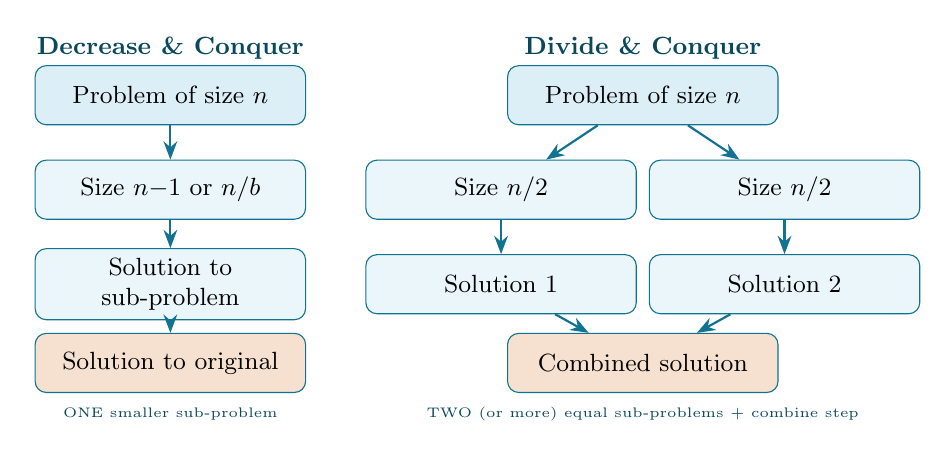
\begin{tikzpicture}[
    box/.style={draw=PrimaryMid,fill=PrimaryLight!30,rounded corners=4pt,
                font=\small,text width=3.2cm,align=center,
                minimum height=0.75cm},
    arr/.style={-{Stealth},PrimaryMid,thick}
  ]
    % Decrease & Conquer column
    \node[box,fill=PrimaryLight!50] (d_prob) at (2.0,3.2) {Problem of size $n$};
    \node[box,fill=PrimaryLight!30] (d_sub)  at (2.0,2.0) {Size $n{-}1$ or $n/b$};
    \node[box,fill=PrimaryLight!30] (d_sol)  at (2.0,0.8) {Solution to sub-problem};
    \node[box,fill=AccentOrange!20] (d_fin)  at (2.0,-0.2){Solution to original};
    \draw[arr] (d_prob)--(d_sub); \draw[arr] (d_sub)--(d_sol);
    \draw[arr] (d_sol)--(d_fin);
    \node[font=\small\bfseries,text=PrimaryDark] at (2.0,3.8)
      {\textbf{Decrease \& Conquer}};
    \node[font=\tiny,text=PrimaryDark,align=center] at (2.0,-0.85)
      {ONE smaller sub-problem};

    % Divide & Conquer column
    \node[box,fill=PrimaryLight!50] (dc_prob) at (8.0,3.2) {Problem of size $n$};
    \node[box,fill=PrimaryLight!30] (dc_l)    at (6.2,2.0) {Size $n/2$};
    \node[box,fill=PrimaryLight!30] (dc_r)    at (9.8,2.0) {Size $n/2$};
    \node[box,fill=PrimaryLight!30] (dc_sl)   at (6.2,0.8) {Solution 1};
    \node[box,fill=PrimaryLight!30] (dc_sr)   at (9.8,0.8) {Solution 2};
    \node[box,fill=AccentOrange!20] (dc_fin)  at (8.0,-0.2){Combined solution};
    \draw[arr] (dc_prob)--(dc_l); \draw[arr] (dc_prob)--(dc_r);
    \draw[arr] (dc_l)--(dc_sl);  \draw[arr] (dc_r)--(dc_sr);
    \draw[arr] (dc_sl)--(dc_fin);\draw[arr] (dc_sr)--(dc_fin);
    \node[font=\small\bfseries,text=PrimaryDark] at (8.0,3.8)
      {\textbf{Divide \& Conquer}};
    \node[font=\tiny,text=PrimaryDark,align=center] at (8.0,-0.85)
      {TWO (or more) equal sub-problems + combine step};
  \end{tikzpicture}
  \end{center}
\end{frame}

\begin{frame}[shrink=12]{Three Variants of Decrease \& Conquer}
  \begin{columns}[T]
    \column{0.55\textwidth}
      \begin{block}{1. Decrease by a constant (usually by 1)}
        $T(n) \to T(n-1) + \text{work}$
        \begin{itemize}
          \item Insertion sort, topological sort
          \item Generating permutations and subsets
        \end{itemize}
      \end{block}
      \vspace{0.3em}
      \begin{block}{2. Decrease by a constant factor (usually by 2)}
        $T(n) \to T(n/2) + \text{work}$
        \begin{itemize}
          \item Binary search, fake-coin problem
          \item Exponentiation by squaring, Russian peasant mult.
        \end{itemize}
      \end{block}
      \column{0.40\textwidth}
      
      \begin{block}{3. Variable-size decrease}
        $T(n) \to T(n') + \text{work}$, where $n'$ varies
        \begin{itemize}
          \item Euclid's GCD, Quickselect, BST operations
        \end{itemize}
      \end{block}
    
      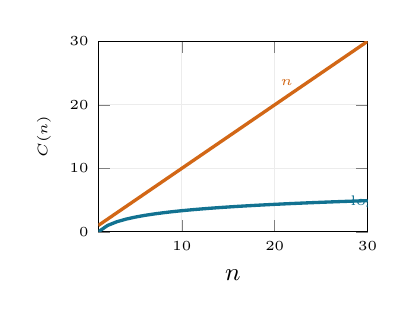
\begin{tikzpicture}
        \begin{axis}[
          width=5.0cm, height=4.0cm,
          xlabel={\small $n$}, ylabel={$C(n)$},
          xmin=1, xmax=30, ymin=0, ymax=30,
          tick label style={font=\tiny},
          label style={font=\tiny},
          no markers, grid=major, grid style={gray!15},
          legend style={font=\tiny,at={(0.98,0.98)},anchor=north east}
        ]
          \addplot[PrimaryMid,very thick,domain=1:30,samples=30]{ln(x)/ln(2)}
            node[pos=0.9,right,font=\tiny]{$\log n$};
          \addplot[AccentOrange,very thick,domain=1:30,samples=30]{x}
            node[pos=0.7,above,font=\tiny]{$n$};
        \end{axis}
      \end{tikzpicture}
      \small Decrease-by-factor $\Rightarrow$ \bigO{\log n}\\
      Decrease-by-1 $\Rightarrow$ \bigO{n} (or \bigO{n\log n})
  \end{columns}
\end{frame}

% ============================================================
\section{Decrease by a Constant}
% ============================================================

\begin{frame}[shrink=12]{Insertion Sort}
  \begin{columns}[T]
    \column{0.50\textwidth}
      \textbf{Idea:} To sort $A[0..n{-}1]$, first sort $A[0..n{-}2]$,
      then \emph{insert} $A[n{-}1]$ into the sorted part.

      \vspace{0.3em}
      \begin{block}{Algorithm}
        \begin{algorithmic}[1]
          \For{$i \gets 1$ \textbf{to} $n{-}1$}
            \State $v \gets A[i]$;\; $j \gets i-1$
            \While{$j \geq 0$ \textbf{and} $A[j] > v$}
              \State $A[j{+}1] \gets A[j]$;\; $j \gets j-1$
            \EndWhile
            \State $A[j{+}1] \gets v$
          \EndFor
        \end{algorithmic}
      \end{block}
    \column{0.45\textwidth}
      \textbf{Trace on $[5,\;3,\;8,\;1]$:}
      \vspace{0.2em}

      \begin{tabular}{cccc}
        \rowcolor{PrimaryDark}\color{white}5&\color{white}3&\color{white}8&\color{white}1 \\
        \rowcolor{PrimaryLight!40}3&5&8&1 \\
        3&5&8&1 \\
        \rowcolor{PrimaryLight!40}1&3&5&8 \\
      \end{tabular}
      \vspace{0.4em}

      \begin{tabular}{lll}
        \toprule
        & \textbf{Comparisons} & \\
        \midrule
        Best (sorted)   & $n-1$ & $\Theta(n)$ \\
        Worst (reverse) & $n(n-1)/2$ & $\Theta(n^2)$ \\
        Average         & $n^2/4$ & $\Theta(n^2)$ \\
        \bottomrule
      \end{tabular}
      \vspace{0.2em}
      Stable: \textcolor{SuccessGreen}{Yes} \quad In-place: \textcolor{SuccessGreen}{Yes}
  \end{columns}
\end{frame}

\begin{frame}[shrink=12]{Topological Sorting}
  \begin{columns}[T]
    \column{0.55\textwidth}
      \begin{block}{Definition}
        A \keyword{topological sort} of a DAG is a linear ordering of
        its vertices such that for every directed edge $(u,v)$,
        $u$ appears before $v$.
      \end{block}
      \vspace{0.3em}
      \textbf{Source-removal algorithm:}
      \begin{enumerate}
        \item Compute in-degree for all vertices
        \item Enqueue all vertices with in-degree $= 0$
        \item Repeat until queue is empty:
          \begin{itemize}
            \item Dequeue vertex $v$, add to sorted list
            \item Decrease in-degree of all neighbors of $v$
            \item Enqueue neighbors whose in-degree becomes 0
          \end{itemize}
        \item If sorted list has $< n$ vertices: \alert{cycle detected}
      \end{enumerate}
      Complexity: \bigO{|V| + |E|}
    \column{0.40\textwidth}
      \textbf{Example: course prerequisites}
      \vspace{0.3em}
      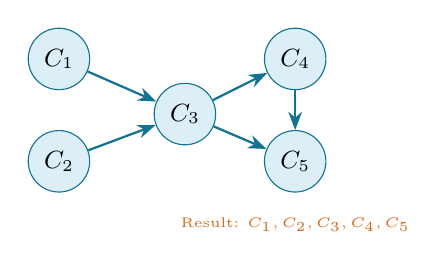
\begin{tikzpicture}[
        nd/.style={circle,draw=PrimaryMid,fill=PrimaryLight!50,
                   font=\bfseries\small,minimum size=0.65cm},
        arr/.style={-{Stealth},PrimaryMid,thick}
      ]
        \node[nd] (c1) at (0,2.5) {$C_1$};
        \node[nd] (c2) at (0,1.2) {$C_2$};
        \node[nd] (c3) at (1.6,1.8) {$C_3$};
        \node[nd] (c4) at (3.0,2.5) {$C_4$};
        \node[nd] (c5) at (3.0,1.2) {$C_5$};
        \draw[arr] (c1)--(c3); \draw[arr] (c2)--(c3);
        \draw[arr] (c3)--(c4); \draw[arr] (c3)--(c5);
        \draw[arr] (c4)--(c5);
        \node[font=\tiny,text=AccentOrange,below=0.2cm of c5]
          {Result: $C_1,C_2,C_3,C_4,C_5$};
      \end{tikzpicture}
      \vspace{0.3em}
      \textbf{In-degrees:}
      $C_1{=}0,\;C_2{=}0,\;C_3{=}2,\;C_4{=}1,\;C_5{=}2$
  \end{columns}
\end{frame}

\begin{frame}[shrink=12]{Generating Subsets}
  \begin{columns}[T]
    \column{0.55\textwidth}
      \textbf{Key observation:} Every subset of $\{a_1,\ldots,a_n\}$
      either contains $a_n$ or it does not.

      \vspace{0.3em}
      \textbf{Recurrence:}
      \[
        \text{Subsets}(n) = \text{Subsets}(n{-}1) \;\cup\;
        \{S \cup \{a_n\} \mid S \in \text{Subsets}(n{-}1)\}
      \]

      \vspace{0.3em}
      \textbf{Bit-string representation:}
      Each subset $\leftrightarrow$ a binary string of length $n$
      (1 = included, 0 = excluded).

      Generate binary numbers from 0 to $2^n{-}1$.
    \column{0.40\textwidth}
      \textbf{All subsets of $\{a_1,a_2,a_3\}$:}
      \vspace{0.2em}

      \begin{tabular}{cc}
        \toprule
        \textbf{Bits} & \textbf{Subset} \\
        \midrule
        000 & $\emptyset$ \\
        001 & $\{a_3\}$ \\
        010 & $\{a_2\}$ \\
        011 & $\{a_2,a_3\}$ \\
        100 & $\{a_1\}$ \\
        101 & $\{a_1,a_3\}$ \\
        110 & $\{a_1,a_2\}$ \\
        111 & $\{a_1,a_2,a_3\}$ \\
        \bottomrule
      \end{tabular}
      \vspace{0.2em}
      \small Total: $2^3 = 8$ subsets \ctag{2^n}
  \end{columns}
\end{frame}

% ============================================================
\section{Decrease by a Constant Factor}
% ============================================================

\begin{frame}[shrink=12]{Binary Search}
  \begin{columns}[T]
    \column{0.50\textwidth}
      \textbf{Problem:} Find key $K$ in a \emph{sorted} array $A[0..n{-}1]$.
      \vspace{0.3em}
      \begin{block}{Algorithm}
        \begin{algorithmic}[1]
          \State $l \gets 0$;\; $r \gets n-1$
          \While{$l \leq r$}
            \State $m \gets \lfloor(l+r)/2\rfloor$
            \If{$K = A[m]$} \Return $m$
            \ElsIf{$K < A[m]$} \State $r \gets m-1$
            \Else \State $l \gets m+1$
            \EndIf
          \EndWhile
          \State \Return $-1$
        \end{algorithmic}
      \end{block}
    \column{0.45\textwidth}
      \textbf{Trace: search for 7 in $[1,3,5,7,9,11]$}
      \vspace{0.2em}

      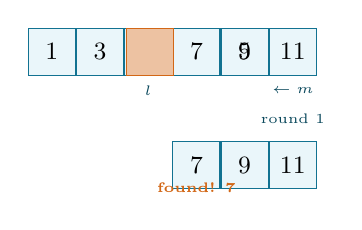
\begin{tikzpicture}[scale=0.9]
        \foreach \i/\v in {0/1,1/3,2/5,3/7,4/9,5/11}{
          \node[draw=PrimaryMid,fill=PrimaryLight!30,minimum size=0.6cm,
                font=\small] at (\i*0.68,0) {\v};
        }
        \node[font=\tiny,text=PrimaryDark] at (1.36,-0.55) {$l$};
        \node[font=\tiny,text=PrimaryDark] at (3.40,-0.55) {$\leftarrow m$};
        \node[font=\tiny,text=PrimaryDark] at (3.40,-0.95) {\alert{round 1}};
        \node[fill=AccentOrange!40,draw=AccentOrange,minimum size=0.6cm,
              font=\small] at (2.04*0.68*1,0) {};
        \node[font=\small] at (2.72,0) {5};
        % Step 2
        \begin{scope}[yshift=-1.6cm]
          \foreach \i/\v in {3/7,4/9,5/11}{
            \node[draw=PrimaryMid,fill=PrimaryLight!30,minimum size=0.6cm,
                  font=\small] at (\i*0.68,0) {\v};
          }
          \node[font=\tiny,text=AccentOrange,below=0.1cm] at (3*0.68,0)
            {\textbf{found! 7}};
        \end{scope}
      \end{tikzpicture}
      \vspace{0.3em}

      $T(n) = T(n/2) + \mathcal{O}(1) \implies$ \bigO{\log n}
  \end{columns}
\end{frame}

\begin{frame}[shrink=12]{Fake Coin Problem}
  \begin{columns}[T]
    \column{0.55\textwidth}
      \textbf{Problem:} Among $n$ identical-looking coins, one is
      counterfeit (lighter). Find it using a balance scale.

      \vspace{0.4em}
      \textbf{Decrease-by-2 (halving):}
      \begin{itemize}
        \item Split coins into two equal groups
        \item Weigh them — the lighter group contains the fake
        \item Recurse on the lighter half
      \end{itemize}
      \[
        W(n) = W(\lfloor n/2\rfloor) + 1 \implies W(n) = \lfloor\log_2 n\rfloor
      \]

      \vspace{0.3em}
      \textbf{Decrease-by-3 (thirds) — even better:}
      \begin{itemize}
        \item Split into three equal groups; weigh two of them
        \item One weighing eliminates $2/3$ of candidates
      \end{itemize}
      \[
        W(n) = W(\lceil n/3\rceil) + 1 \implies W(n) = \lceil\log_3 n\rceil
      \]
    \column{0.40\textwidth}
      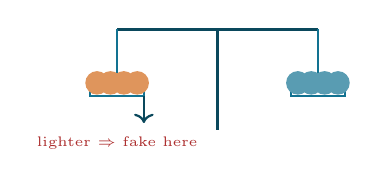
\begin{tikzpicture}[scale=0.85]
        % Balance
        \draw[PrimaryDark,very thick] (1.5,2) -- (1.5,0.5);
        \draw[PrimaryDark,very thick] (0,2) -- (3,2);
        \draw[PrimaryMid,thick] (0,2) -- (0,1.2);
        \draw[PrimaryMid,thick] (3,2) -- (3,1.2);
        % Pans
        \draw[PrimaryMid,thick] (-0.4,1.2) rectangle (0.4,1.0);
        \draw[PrimaryMid,thick] (2.6,1.2) rectangle (3.4,1.0);
        % Coins
        \foreach \x in {-0.3,-0.1,0.1,0.3}{
          \fill[AccentOrange!70] (\x,1.2) circle(5pt);
        }
        \foreach \x in {2.7,2.9,3.1,3.3}{
          \fill[PrimaryMid!70] (\x,1.2) circle(5pt);
        }
        % Tilt
        \draw[PrimaryDark,thick,->] (0.4,1.0) -- (0.4,0.6);
        \node[font=\tiny,text=AlertRed] at (0,0.3) {lighter $\Rightarrow$ fake here};
      \end{tikzpicture}
      \vspace{0.4em}
      \begin{block}{Key insight}
        Decrease-by-3 requires $\lceil\log_3 n\rceil$ weighings,
        fewer than $\lfloor\log_2 n\rfloor$ for $n > 3$.
      \end{block}
  \end{columns}
\end{frame}

\begin{frame}[shrink=12]{Russian Peasant Multiplication}
  \textbf{Problem:} Compute $m \times n$ using only halving, doubling, and addition.

  \vspace{0.3em}
  \begin{columns}[T]
    \column{0.48\textwidth}
      \textbf{Recurrence:}
      \[
        m \cdot n =
        \begin{cases}
          \dfrac{m}{2} \cdot 2n & m \text{ even} \\[6pt]
          \dfrac{m-1}{2} \cdot 2n + n & m \text{ odd}
        \end{cases}
      \]
      \vspace{0.2em}
      Add $n$ whenever $m$ is \emph{odd}; always halve $m$ and double $n$.
    \column{0.48\textwidth}
      \textbf{Example: $20 \times 26$}
      \vspace{0.2em}

      \begin{tabular}{rrr}
        \toprule
        $m$ & $n$ & add? \\
        \midrule
        20 & 26  & — \\
        10 & 52  & — \\
         5 & 104 & \textcolor{SuccessGreen}{$+104$} \\
         2 & 208 & — \\
         1 & 416 & \textcolor{SuccessGreen}{$+416$} \\
        \bottomrule
      \end{tabular}
      \vspace{0.2em}
      $\text{Result} = 104 + 416 = \highlight{520}$\ctag{\log n}
  \end{columns}
\end{frame}

% ============================================================
\section{Variable-Size Decrease}
% ============================================================

\begin{frame}[shrink=12]{Quickselect — Finding the $k$-th Smallest}
  \begin{columns}[T]
    \column{0.55\textwidth}
      \textbf{Problem:} Find the $k$-th smallest element in an unsorted
      array of $n$ elements (e.g., the \emph{median}).

      \vspace{0.3em}
      \textbf{Lomuto partition around pivot $p$ (first element):}
      \[
        \underbrace{A[0]\cdots A[s{-}1]}_{\leq p}
        \;\; p \;\;
        \underbrace{A[s{+}1]\cdots A[n{-}1]}_{\geq p}
      \]
      After partition, pivot is at index $s$:
      \begin{itemize}
        \item If $s = k-1$: \textbf{done}, return $A[s]$
        \item If $s > k-1$: recurse on left part
        \item If $s < k-1$: recurse on right part
      \end{itemize}
    \column{0.40\textwidth}
      \textbf{Complexities:}
      \begin{tabular}{ll}
        \toprule
        Case & Complexity \\
        \midrule
        Best  & $\Theta(n)$ \\
        Worst & $\Theta(n^2)$ \\
        Average & $\Theta(n)$ \\
        \bottomrule
      \end{tabular}
      \vspace{0.4em}
      \begin{exampleblock}{Real-world use}
        Finding the median salary among 1 million records
        \emph{without} sorting them all — used in statistics,
        databases, and data science pipelines.
      \end{exampleblock}
  \end{columns}
\end{frame}

\begin{frame}[shrink=20]{Interpolation Search}
  \begin{columns}[T]
    \column{0.55\textwidth}
      \textbf{Idea:} Like binary search, but probe position is estimated
      from the \emph{value} of the key, assuming uniform distribution.
      \vspace{0.2em}
      \begin{block}{Algorithm sketch}
        \begin{algorithmic}[1]
          \While{$l \leq r$ \textbf{and} $v \in [A[l],A[r]]$}
            \State compute probe position $x$ via formula
            \If{$A[x] = v$} \Return $x$
            \ElsIf{$A[x] < v$} \State $l \gets x+1$
            \Else \State $r \gets x-1$
            \EndIf
          \EndWhile
          \State \Return $-1$
        \end{algorithmic}
      \end{block}
    \column{0.40\textwidth}
     \vspace{0.2em}
          \[
        x = l + \left\lfloor \frac{(v - A[l])(r-l)}{A[r]-A[l]} \right\rfloor
      \]
       \vspace{0.2em}
      \begin{tabular}{ll}
        \toprule
        Case & Complexity \\
        \midrule
        Best (uniform) & $\mathcal{O}(\log\log n)$ \\
        Worst & $\mathcal{O}(n)$ \\
        Average (uniform) & $\mathcal{O}(\log\log n)$ \\
        \bottomrule
      \end{tabular}
      \vspace{0.4em}
      \begin{alertblock}{When to prefer over binary search}
        Only for \emph{very large} sorted arrays with
        \emph{uniformly distributed} values.
        Otherwise binary search is safer.
      \end{alertblock}
  \end{columns}
\end{frame}

% ============================================================
\section{Divide \& Conquer — Introduction}
% ============================================================

\begin{frame}[shrink=18]{Divide \& Conquer: The General Recurrence}
  \begin{columns}[T]
    \column{0.55\textwidth}
      \begin{block}{Recurrence}
        $T(n) = a\,T(n/b) + f(n)$, \quad $f(n)\in\Theta(n^d)$, $d\geq 0$
      \end{block}
      \vspace{0.3em}
      \begin{block}{Master Theorem}
        \[
          T(n) \in
          \begin{cases}
            \textcolor{SuccessGreen}{\Theta(n^d)}          & \text{if } a < b^d \;(\text{combine dominates})\\
            \textcolor{AccentOrange}{\Theta(n^d \log n)}   & \text{if } a = b^d \;(\text{balanced})\\
            \textcolor{AlertRed}{\Theta(n^{\log_b a})}     & \text{if } a > b^d \;(\text{recursion dominates})
          \end{cases}
        \]
      \end{block}
      \vspace{0.3em}
      \scriptsize
      \begin{tabular}{lrrrcc}
        \toprule
        \textbf{Recurrence} & $a$ & $b$ & $d$ & \textbf{Case} & \textbf{Result} \\
        \midrule
        \rowcolor{AlertRed!10}   $3T(n/2)+n$   & 3 & 2 & 1 & $a>b^d$ & $\Theta(n^{\log_2 3})\approx\Theta(n^{1.585})$ \\
        \rowcolor{SuccessGreen!10}$3T(n/2)+n^2$ & 3 & 2 & 2 & $a<b^d$ & $\Theta(n^2)$ \\
        \rowcolor{AccentOrange!10}$4T(n/2)+n^2$ & 4 & 2 & 2 & $a=b^d$ & $\Theta(n^2\log n)$ \\
        \rowcolor{AccentOrange!10}$2T(n/2)+n$   & 2 & 2 & 1 & $a=b^d$ & $\Theta(n\log n)$ \\
        \bottomrule
      \end{tabular}
    \column{0.40\textwidth}
      \begin{alertblock}{Does not apply when:}
        \begin{itemize}
          \item $a < 1$ or $d < 0$
          \item $f(n)$ is not polynomial
          \item $a$ is not a constant
        \end{itemize}
      \end{alertblock}
      \vspace{0.4em}
      \begin{exampleblock}{Memory aid}
        Compare the \emph{branching factor} $a$ with the \emph{shrink–work ratio} $b^d$:
        \begin{itemize}
          \item $a < b^d$: work at root dominates
          \item $a = b^d$: cost spreads evenly
          \item $a > b^d$: leaves dominate
        \end{itemize}
      \end{exampleblock}
  \end{columns}
\end{frame}

% ============================================================
\section{Mergesort}
% ============================================================

\begin{frame}[shrink=12]{Mergesort — Algorithm}
  \begin{columns}[T]
    \column{0.50\textwidth}
      \textbf{Idea:} Split array in half, sort each half recursively,
      then \emph{merge} the two sorted halves.
      \vspace{0.3em}
      \begin{block}{Mergesort}
        \begin{algorithmic}[1]
          \Require Array $A[0..n{-}1]$
          \If{$n > 1$}
            \State split $A$ into $B[0..\lfloor n/2\rfloor{-}1]$ and $C[\ldots]$
            \State \textsc{Mergesort}($B$)
            \State \textsc{Mergesort}($C$)
            \State \textsc{Merge}($B, C, A$)
          \EndIf
        \end{algorithmic}
      \end{block}
      \vspace{0.2em}
      \textbf{Merge}: compare heads of $B$ and $C$, copy smaller.
      Runs in $\Theta(p+q)$ where $|B|=p$, $|C|=q$.
    \column{0.45\textwidth}
      \textbf{Recursion tree for $n=8$:}
      \vspace{0.2em}
      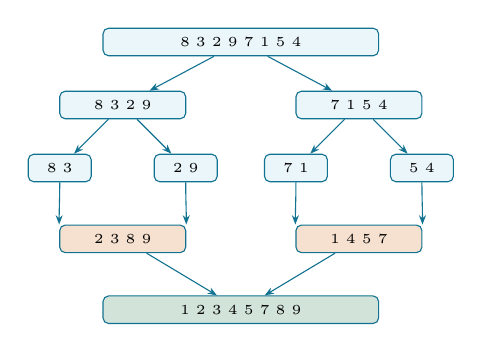
\begin{tikzpicture}[
        nd/.style={draw=PrimaryMid,fill=PrimaryLight!30,rounded corners=2pt,
                   font=\tiny,minimum width=0.7cm,minimum height=0.35cm},
        arr/.style={-{Stealth[scale=0.7]},PrimaryMid}
      ]
        \node[nd,minimum width=3.5cm] (r) at (3.0,3.0) {8 3 2 9 7 1 5 4};
        \node[nd,minimum width=1.6cm] (l1) at (1.5,2.2) {8 3 2 9};
        \node[nd,minimum width=1.6cm] (r1) at (4.5,2.2) {7 1 5 4};
        \node[nd,minimum width=0.8cm] (l2) at (0.7,1.4) {8 3};
        \node[nd,minimum width=0.8cm] (l3) at (2.3,1.4) {2 9};
        \node[nd,minimum width=0.8cm] (r2) at (3.7,1.4) {7 1};
        \node[nd,minimum width=0.8cm] (r3) at (5.3,1.4) {5 4};
        \draw[arr] (r)--(l1); \draw[arr] (r)--(r1);
        \draw[arr] (l1)--(l2); \draw[arr] (l1)--(l3);
        \draw[arr] (r1)--(r2); \draw[arr] (r1)--(r3);
        % Merge results
        \node[nd,minimum width=1.6cm,fill=AccentOrange!20] (m1) at (1.5,0.5) {2 3 8 9};
        \node[nd,minimum width=1.6cm,fill=AccentOrange!20] (m2) at (4.5,0.5) {1 4 5 7};
        \node[nd,minimum width=3.5cm,fill=SuccessGreen!20] (fin) at (3.0,-0.4) {1 2 3 4 5 7 8 9};
        \draw[arr] (l2)to[out=270,in=90](m1.north west);
        \draw[arr] (l3)to[out=270,in=90](m1.north east);
        \draw[arr] (r2)to[out=270,in=90](m2.north west);
        \draw[arr] (r3)to[out=270,in=90](m2.north east);
        \draw[arr] (m1)--(fin); \draw[arr] (m2)--(fin);
      \end{tikzpicture}
  \end{columns}
\end{frame}

\begin{frame}[shrink=12]{Mergesort — Analysis}
  \begin{columns}[T]
    \column{0.55\textwidth}
      \textbf{Recurrence:}
      \[
        T(n) = 2T(n/2) + \Theta(n),\quad T(1)=\mathcal{O}(1)
      \]
      Master Theorem: $a=2,\;b=2,\;d=1 \implies a=b^d$
      \[
        \boxed{T(n) = \Theta(n\log n)}
      \]
      \vspace{0.2em}
      \textbf{All cases are $\Theta(n\log n)$} (the merge always takes $\Theta(n)$).

      \vspace{0.3em}
      Number of comparisons (worst case) $\approx n\log_2 n$, close to the
      information-theoretic lower bound $\lceil\log_2 n!\rceil \approx n\log_2 n - 1.44n$.
    \column{0.40\textwidth}
      \begin{tabular}{lll}
        \toprule
        & \textbf{Mergesort} & \textbf{Bubble} \\
        \midrule
        Best     & $\Theta(n\log n)$ & $\Theta(n)$ \\
        Worst    & $\Theta(n\log n)$ & $\Theta(n^2)$ \\
        Average  & $\Theta(n\log n)$ & $\Theta(n^2)$ \\
        Space    & $\Theta(n)$ & $\Theta(1)$ \\
        Stable   & Yes & Yes \\
        \bottomrule
      \end{tabular}
      \vspace{0.3em}
      \begin{alertblock}{Trade-off}
        Mergesort is not \emph{in-place} — it requires
        $\Theta(n)$ extra space for the merge step.
        Prefer it for \emph{linked lists}.
      \end{alertblock}
  \end{columns}
\end{frame}

% ============================================================
\section{Quicksort}
% ============================================================

\begin{frame}[shrink=12]{Quicksort — Algorithm}
  \begin{columns}[T]
    \column{0.50\textwidth}
      \textbf{Idea:} Choose a \emph{pivot}, partition the array so that
      all elements $\leq$ pivot come first, then recursively sort
      both parts.
      \vspace{0.3em}
      \begin{block}{Quicksort}
        \begin{algorithmic}[1]
          \Require Subarray $A[l..r]$
          \If{$l < r$}
            \State $s \gets \textsc{Partition}(A[l..r])$
            \State \textsc{Quicksort}($A[l..s{-}1]$)
            \State \textsc{Quicksort}($A[s{+}1..r]$)
          \EndIf
        \end{algorithmic}
      \end{block}
      \vspace{0.2em}
      \textbf{Hoare partition} scans inward from both ends,
      swapping out-of-place elements until the pointers cross.
    \column{0.45\textwidth}
      \textbf{Pivot strategies:}
      \begin{itemize}
        \item \keyword{First element} — simple, \alert{bad on sorted input}
        \item \keyword{Median-of-three} — good average behaviour
        \item \keyword{Random element} — avoids adversarial inputs
      \end{itemize}
      \vspace{0.4em}
      \textbf{Complexities:}
      \begin{tabular}{ll}
        \toprule
        Best / Average & $\Theta(n\log n)$ \\
        Worst          & $\Theta(n^2)$ \\
        Space (avg)    & $\mathcal{O}(\log n)$ stack \\
        Stable         & No \\
        In-place       & Yes \\
        \bottomrule
      \end{tabular}
  \end{columns}
\end{frame}

\begin{frame}[shrink=12]{Quicksort vs Mergesort}
  \begin{columns}[T]
    \column{0.55\textwidth}
      \begin{tabular}{lll}
        \toprule
        \textbf{Property} & \textbf{Quicksort} & \textbf{Mergesort} \\
        \midrule
        Average time   & $\Theta(n\log n)$ & $\Theta(n\log n)$ \\
        Worst time     & $\Theta(n^2)$ & $\Theta(n\log n)$ \\
        Extra space    & $\mathcal{O}(\log n)$ & $\Theta(n)$ \\
        In-place       & \textcolor{SuccessGreen}{Yes} & \alert{No} \\
        Stable         & \alert{No} & \textcolor{SuccessGreen}{Yes} \\
        Cache perf.    & Better & Good \\
        \bottomrule
      \end{tabular}
    \column{0.40\textwidth}
      \begin{exampleblock}{Guideline}
        \begin{itemize}
          \item Prefer \keyword{Quicksort} for arrays in practice
                (better cache behaviour, in-place)
          \item Prefer \keyword{Mergesort} for linked lists
                (in-place merge in $\mathcal{O}(1)$ extra space)
          \item Use \keyword{Timsort} (hybrid) for general-purpose
                libraries (Python, Java)
        \end{itemize}
      \end{exampleblock}
  \end{columns}
\end{frame}

% ============================================================
\section{Binary Trees \& Closest Pair}
% ============================================================

\begin{frame}[shrink=12]{Binary Tree Traversals}
  \begin{columns}[T]
    \column{0.50\textwidth}
      A \keyword{binary tree} is naturally processed by Divide \& Conquer:
      divide into root + left subtree + right subtree.

      \vspace{0.4em}
      \begin{block}{Height of a binary tree}
        \begin{algorithmic}[1]
          \If{$T = \emptyset$} \Return $-1$ \EndIf
          \State \Return $\max(\text{Height}(T_L),\,\text{Height}(T_R)) + 1$
        \end{algorithmic}
      \end{block}

      \textbf{Traversal orders:}
      \begin{itemize}
        \item \concept{Preorder}: root, left, right
        \item \concept{Inorder}: left, root, right ← produces sorted order for BST
        \item \concept{Postorder}: left, right, root
      \end{itemize}
      All traversals: $\Theta(n)$
    \column{0.45\textwidth}
      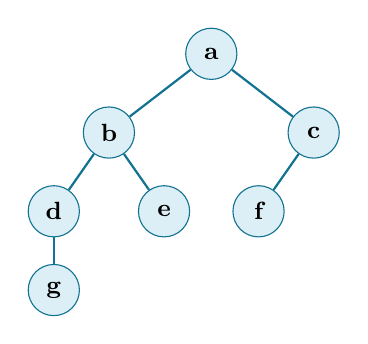
\begin{tikzpicture}[
        nd/.style={circle,draw=PrimaryMid,fill=PrimaryLight!50,
                   font=\bfseries\small,minimum size=0.65cm},
        arr/.style={draw=PrimaryMid,thick}
      ]
        \node[nd] (a) at (2.5,3.2) {a};
        \node[nd] (b) at (1.2,2.2) {b};
        \node[nd] (c) at (3.8,2.2) {c};
        \node[nd] (d) at (0.5,1.2) {d};
        \node[nd] (e) at (1.9,1.2) {e};
        \node[nd] (f) at (3.1,1.2) {f};
        \node[nd] (g) at (0.5,0.2) {g};
        \draw[arr] (a)--(b); \draw[arr] (a)--(c);
        \draw[arr] (b)--(d); \draw[arr] (b)--(e);
        \draw[arr] (c)--(f);
        \draw[arr] (d)--(g);
      \end{tikzpicture}
      \vspace{0.2em}
      \begin{tabular}{ll}
        Preorder:  & a, b, d, g, e, c, f \\
        Inorder:   & g, d, b, e, a, f, c \\
        Postorder: & g, d, e, b, f, c, a \\
      \end{tabular}
  \end{columns}
\end{frame}

\begin{frame}[shrink=12]{Closest Pair — Divide \& Conquer}
  \begin{columns}[T]
    \column{0.55\textwidth}
      \textbf{Problem:} Find the two closest points in $n$ points
      in the plane. Brute force: $\mathcal{O}(n^2)$.

      \vspace{0.3em}
      \textbf{D\&C algorithm sketch:}
      \begin{enumerate}
        \item Sort points by $x$-coordinate
        \item Split at median $x$ into $P_L$ and $P_R$
        \item Recurse: $d_L = \text{closestPair}(P_L)$,
              $d_R = \text{closestPair}(P_R)$
        \item $d = \min(d_L, d_R)$
        \item Check the "strip" of width $2d$ around the dividing line
              (at most 8 point-pairs per strip element)
      \end{enumerate}

      \textbf{Recurrence:}
      $T(n) = 2T(n/2) + \mathcal{O}(n)$

      $\implies T(n) = \mathcal{O}(n\log n)$
    \column{0.40\textwidth}
      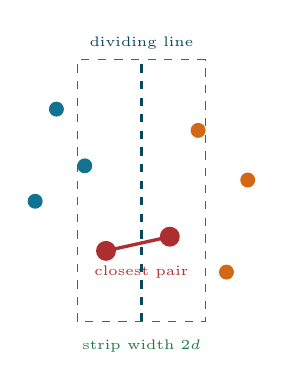
\begin{tikzpicture}[scale=0.9]
        \draw[PrimaryDark,dashed,thick] (2.0,-0.2) -- (2.0,3.5)
          node[above,font=\tiny]{dividing line};
        % Points left
        \foreach \x/\y in {0.5/1.5,0.8/2.8,1.5/0.8,1.2/2.0}{
          \fill[PrimaryMid] (\x,\y) circle(3pt);}
        % Points right
        \foreach \x/\y in {2.4/1.0,2.8/2.5,3.5/1.8,3.2/0.5}{
          \fill[AccentOrange] (\x,\y) circle(3pt);}
        % Closest pair across boundary
        \draw[AlertRed,very thick] (1.5,0.8) -- (2.4,1.0);
        \fill[AlertRed] (1.5,0.8) circle(4pt);
        \fill[AlertRed] (2.4,1.0) circle(4pt);
        \draw[SuccessGreen,dashed] (1.1,-0.2) rectangle (2.9,3.5);
        \node[font=\tiny,text=SuccessGreen] at (2.0,-0.55) {strip width $2d$};
        \node[font=\tiny,text=AlertRed] at (2.0,0.5) {closest pair};
      \end{tikzpicture}
  \end{columns}
\end{frame}

% ── Chapter Summary ──────────────────────────────────────────
\begin{frame}[shrink=12]{Chapter 4 Summary}
  \begin{columns}[T]
    \column{0.55\textwidth}
      \textbf{Decrease \& Conquer:}
      \begin{tabular}{lll}
        Insertion sort & $\mathcal{O}(n^2)$ worst \\
        Topological sort & $\mathcal{O}(|V|+|E|)$ \\
        Binary search & $\mathcal{O}(\log n)$ \\
        Quickselect & $\mathcal{O}(n)$ avg \\
      \end{tabular}
      \vspace{0.3em}

      \textbf{Divide \& Conquer:}
      \begin{tabular}{lll}
        Mergesort & $\Theta(n\log n)$ & all cases \\
        Quicksort & $\Theta(n\log n)$ & avg \\
        Closest pair & $\Theta(n\log n)$ & \\
        Tree traversal & $\Theta(n)$ & \\
      \end{tabular}
    \column{0.40\textwidth}
      \begin{block}{Master Theorem}
        $T(n)=aT(n/b)+\Theta(n^d)$:
        \begin{itemize}
          \item $a < b^d$: $\Theta(n^d)$
          \item $a = b^d$: $\Theta(n^d\!\log n)$
          \item $a > b^d$: $\Theta(n^{\log_b a})$
        \end{itemize}
      \end{block}
      \vspace{0.2em}
      \begin{block}{Next chapter}
        \textbf{Chapter 5:} Transform \& Conquer —
        presorting, balanced trees, heaps, and
        problem reduction (including linear programming).
      \end{block}
  \end{columns}
\end{frame}

\end{document}
